% !TeX spellcheck = en_US
\documentclass[]{TAACpaper}
\usepackage[linesnumbered,boxed]{algorithm2e}
\pagestyle{plain}
\begin{document}

%This is the comment. Further under the text features of use of style of theses are described

%We are specifying language of the paper
\selectlanguage{russian}
\def\dd#1#2{\frac{\partial#1}{\partial#2}}
\section{
``Исследование  настроечных параметров алгоритма поиска с запретами и его модификация для решения курьерской задачи маршрутизации.'' 
}

\authors{
L.~Lyubchik, R.~Shafeyev 
}

\abstract{
%%%%%%%%%%%%%%% You have to insert abstract of your paper here

В статье рассматривается задача маршрутизации курьерской доставки  с долгим сроком службы, для которой была построена дискретная модель и вычислительная схема, в основу которой был положен алгоритм поиска с запретами. Эффективность схемы предложенного алгоритма была проверена на задачах большой размерности, которые были составлены на базе известных модельных задачах маршрутизации на транспорте различных классов.
}

%%%%%%%%%%%%%%% To define new section use a command \subsection
% We are defining "Introduction" here
\subsection{Introduction}
%%%%% Paragraph text. To separate paragraphs use empty lines.
Одним из средств экономии ресурсов при транспортировке грузов является применение систем поддержки принятия решений в сфере транспортной логистики. Одной из ключевых функций систем поддержки принятия решений в сфере транспортной логистики является возможность расчета и построения эффективных с точки зрения стоимости объезда маршрутов различного назначения на транспортной сети. Математическая формулировка этой задачи широко известно как задача маршрутизации транспорта. Существует ряд разновидностей ЗМТ с различными дополнительными условиями, которые позволяют учитывать грузоподъемность транспортных средств и другие ограничения для более полного представления деталей реальной действительности.

Данная статья посвящена рассмотрению задачи курьерской маршрутизации, которая является подзадачей ЗМТ. Данная задача состоит в нахождении маршрутов для посещения заданного множества адресов некоторым количеством единиц транспортных средств. Такая проблема наиболее часто встречается среди компаний, выполняющих развозки товара от отправителя к получателю. 

Автоматизация процесса планирования маршрутов будет актуальной для:  интернет-магазинов, крупных оптовых компаний (например, для развозки товаров, которые быстро портятся или оптимизации схемы доставки товаров в пункты назначения), фирм с целью организации допоставок в магазины. Практическое применение задачи можно встретить в сфере транспортировки пациентов между корпусами поликлиники\cite{Beaudry, Kergosien}, доставке газет и журналов, доставки топлива в частные дома \cite{Sarak}. Решение рассматриваемой задачи также имеет практическое применение в системах вертолетных перевозок людей между морскими нефтяными платформами \cite{Romero}.

В последнее время все больше людей пользуются услугами курьерских служб.  Обычно заявки формируются днем ранее и
перед диспетчером полный список заявок, которые необходимо выполнить в кратчайшие сроки. Тематическое исследование провел Attanasio(2007) \cite{Attanasio}, в котором описал преимущества использования компьютерных методов перед человеческой диспетчеризацией. В своей работе он рассмотрел примеры работы eCourier Ltd, лондонской компании, которая предлагает курьерские услуги. Их клиентами в основном являются юридические фирмы, финансовые учреждения, рекламные агентства и другие организации, которые заинтересованы в быстрой доставке товаров или оригинальных подписях на документах. После того как все заявки на конкретный момент времени сформированы, необходимо составить такой маршрут, который удовлетворял бы требованиям заказчиков. В зависимости от уровня обслуживания, который был задан клиентом, курьер может объединить или ни его доставку с другими, то есть это означает, что товары могут быть доставлены по очереди, или курьер может выполнить ускоренную доставку. 

Компании, которые предлагают курьерские услуги достаточно часто имеют смешанный парк транспортных средств, который состоит из велосипедов, мотоциклов, автомобилей и небольших грузовиков. В зависимости от типа запроса, расположение и временных окон будет выбран тот вид транспортного средства, который сможет выполнить заказ в кратчайшие сроки. Исследования \cite{Attanasio} показали, что использование компьютерных методов, в том числе алгоритмов оптимизации, были очень выгодными для курьерских компаний.

Таким образом, использование автоматизированной системы позволяет улучшить качество обслуживания, время доставки, повысить курьерскую эффективность и сократить расходы на доставку, тем самым обеспечить повышение конкурентного преимущества.

\subsection{Постановка задачи}
Пусть $C,dim(C)=n$ -- множество транспортных средств, $Q,dim(Q)=m$ -- множество запросов клиентов, которые требуется обработать на текущий момент времени.

Предположим, что следующая информация известна о транспортных средствах из множества $C$: \\
$\vec{P}_c$ -- местоположение ТС, $c \in C$;\\
$L_c$ -- грузоподъемность ТС, $c \in C$.

Пусть $S$ -- множество отправителей груза, ($dim(S) = dim(Q) = m$), $R$ -- множество получателей, $dim(R) = dim(Q) = m$. Тогда каждый клиентский запрос $q \in Q$ включает в себя следующую информацию:\\
$s_q$ -- отправитель груза клиента, $s \in S$; \\
$r_q$ -- получатель клиентского груза, $r \in R$; \\
$\vec{P}_{s_q}$ -- Местоположение отправителя;\\
$\vec{P}_{r_q}$ -- Местоположение получателя; \\
$w_q$ -- клиентский груз, который требуется перевезти от отправителя к получателю; \\
$[t_{s}^{q}, t_{s}^{q}+ \Delta{t_{s}^{q}}]$ -- временное окно, в течение которого нужно забрать груз у отправителя;\\ 
$[t_{r}^{q}, t_{r}^{q}+ \Delta{t_{r}^{q}}]$ -- временное окно, в течение которого нужно доставить груз получателю.
 
Таким образом, каждая заявка может быть представлена в виде кортежа:
\begin{equation}
\forall q \in Q: \exists q = (s_q,r_q, \vec{P}_{s_q}, \vec{P}_{r_q}, w_q, t_{s}^{q}, \Delta{t_{s}^{q}}, t_{r}^{q}, \Delta{t_{r}^{q}})
\end{equation}
Для того, чтобы оценить стоимость перевозки между пунктами назначения, определим функцию стоимости $\Omega$:
\begin{equation}
\forall i,j \in S \cup R: \exists \Omega_{i,j} = \Omega(\vec{P}_i,\vec{P}_j)
\end{equation}

Необходимо построить оптимальные маршруты движения транспортных средств для перевозки грузов от отправителя к получателю для всех клиентских запросов.

\begin{figure}[h]
	\hfil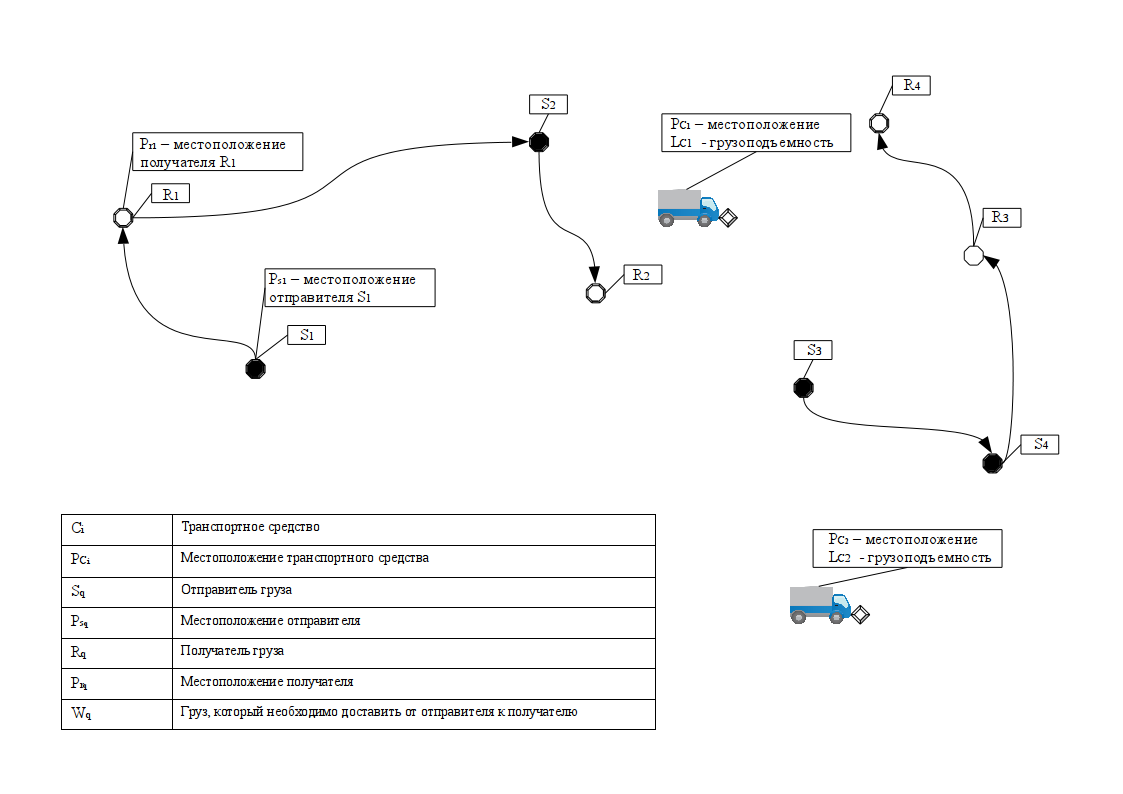
\includegraphics[height=4.0in]{images/scheme}\hfil
	\caption
	{
		Example of the Routing Delivery Problem.
	}
	\label{aba:fig1}
\end{figure}

\subsection{Дискретная модель}
Задачу маршрутизации можно представить в виде ориентированного графа $G=G(V,E)$. Пусть множество $V=C\cup{S}\cup{R}$ -- узлы графа $G$,  состоящее из элементов множеств транспортных средств $C$, отправителей $S$ и получателей $R$. $E$ -- динамическое множество дуг графа $G$, такое, что:
\begin{equation}
\forall e(X) \in E: e(X) = (v_i,v_j), \exists v_i \in V, v_j \in V/C
\end{equation}

Пусть $X = \{X^k\}^n_{k=1}$ представляет собой последовательность матриц для каждого ТС $k \in C$. Элементы матрицы принимают следующие значения:
\begin{equation}
  x^{(k)}_{i,j} = 
    \begin{cases}
	  1,&\text{АТС $k \in C$ движется с узла $i$ в вершину $j$}\\
	  0,&\text{в противном случае.}
    \end{cases}
\end{equation}
где: $i\in{V/C \cup {k}}, j \in V/C$.

Введем вектор переменных $ \vec{Y}  ^ k(X) $ для каждого транспортного средства  $ k \ in C $. Векторные элементы принимают следующие значения:
\begin{equation}
\vec{y}^{(k)}_{j}(X) = 
\begin{cases}
1,&\text{Запрос $j \in Q$ обслуживается ТС $k \in C$}\\
0,&\text{в противном случае}
\end{cases}
\end{equation}
где: $i\in{V/C \cup {k}}, j \in V/C$.


Пусть $t^k_j(X^{(k)})$ -- время прибытия автомобиля $k \in C$ в пункт назначения $j \in S \cup R$. 

Целевая функция принимает следующий вид:
\begin{equation} \label{main_objective}
  F(X) = 
    \sum_{k \in C}
     \sum_{i,j\cup{V}} 
     \Omega_{ij} \cdot x_{ij}^{(k)} 
     \to min
\end{equation}

Наложим ограничения на целевую функцию  (\ref{main_objective}) для обеспечения непрерывности маршрутов:
\begin{align} 
& \sum_{k \in C}\sum_{j \in S \cup R}x^{(k)}_{i,j} \leq 1, 
\forall i \in V \label{main_cond_1}\\
& \sum_{k \in C}\sum_{i \in S \cup R \cup \{k\} } x^{(k)}_{i,j} = 1, 
\forall j \in S \cup R \label{main_cond_2}\\
& \sum_{i \in S \cup R \cup \{k\} } x^{(k)}_{i,\omega} - 
\sum_{j \in S \cup R} x^{(k)}_{\omega,j} \leq 1, 
\forall \omega \in S \cup R,  \forall k \in C \label{main_cond_3}\\
&  \sum_{i \in S \cup R / Z}\sum_{j \in Z } x^{(k)}_{i,j} > 0, 
Z=\{z \in Z: \sum_{j \in S \cup R}x^{(k)}_{j,z}>0 \}  ,\forall k \in C \label{main_cond_4}
\end{align}

Ограничение (\ref{main_cond_1}) запрещает, чтобы у узла графа $G$ было более чем одна выходящая дуга. Ограничение (\ref {main_cond_2}) запрещает узлу иметь более чем одну входную дугу. Ограничение (\ref {main_cond_3}) указывает на то, что у узла количество входных дуг не может быть меньше количества выходных дуг (это ограничение учитывает тот факт, что транспортное средство может покинуть пункт назначения, если только он посетил этот узел). Ограничение (\ref {main_cond_4}) исключает локальные циклы.

Следующие ограничения синхронизируют значения переменных $X$ и $ \Vec{у} $ для каждого запроса $ Q \ в Q $ и запрещают посещение получателя перед отправителем:

\begin{align} 
& x^{(k)}_{s_q} + x^{(k)}_{r_q} = 2 \cdot y^{(k)}_{q}(X), \forall k \in C, q \in Q  \\
& y^{(k)}_{q}(X) \cdot (\tilde{t}^k_{r_q}(X^{(k)})-\tilde{t}^k_{s_q}(X^{(k)})\ge{0}, \forall k \in C, q \in Q
\end{align}

Определим ограничения для учета грузоподъемности транспортных средств и временные окна:
\begin{align} 
& \sum_{j\in{Q}} \omega_j \cdot y_{j}^{k} \leq L_k, \forall{k}\in{C}\\
& t_{s}^{q} \leq \tilde{t}^k_{s_q}(X^{(k)} \leq t_{s}^{q}+ \Delta{t_{s}^{q}}, \forall q \in Q, \label{tws_cond} \\
& t_{r}^{q} \leq \tilde{t}^k_{r_q}(X^{(k)} \leq t_{r}^{q}+ \Delta{t_{r}^{q}}, \forall q \in Q, \label{twr_cond}
\end{align}



\subsection{Описание алгоритма}
Представим множество матриц $\{X^k\}$ в виде вектора, определенного на гиперкубе $E^\eta=\{0.1\}^\eta$, где $\eta=n\cdot(2m+1)\cdot 2m$. Цель задачи состоит в минимизации следующей целевой функции:
		
\begin{align} 
& F(\vec{u})\to min,\vec{u}\in E^{\eta}
\end{align}	

Обозначим через $\delta(\vec{u},\vec{v})$ расстояние Хэмминга между $\vec{u}$ и $\vec{v}$. Через $N_l(\vec{u})$ обозначим окрестность точки $\vec{u}$ дариусом $l$ \cite{vrp_shafeyev}:
\begin{align} 
& N_l(\vec{u})=\{\vec{v} \in E^{\eta}:\delta(\vec{u},\vec{v})\le l \}, l=\bar{1,\eta}
\end{align}	


При $ л = \ ETA $ множество $ N_l (\ VEC {и}) $ для любого вектора $ \ VEC {и} $ совпадает с множеством $ E ^ {\ эты} $ и быть в этой окрестности вектора с минимальным значение целевой функции эквивалентна решению исходной задачи. Стандартный алгоритм Локальный алгоритм поиска начинается с выбранного случайным образом вектор $ \ VEC {и ^ 0} $.
На $ I $ шаг алгоритма перехода от текущего вектора в соседней, что минимальное значение целевой функции в окрестности данного вектора:

Когда $l=\eta$, тогда множество $ N_l(\vec{u})$ для любого вектора $\vec{u}$ совпадает с множеством $E^{\eta}$  и поиск в этой окрестности минимума эквивалентно решению исходной задачи. Классический алгоритм локального поиска начинает поиск оптимума с  инициализации вектора $\vec{u^0}$.
На $i$ шаге алгоритма  алгоритма выполняется перемещение текущего вектора в минимум его окрестности:
\begin{align} 
& F(\vec{u}^{i+1})=min\{F(\vec{v}):\vec{v} \in N_l(\vec{u}^i)\}
\end{align}	

Алгоритм завершается в локальном оптимуме, когда $F(\vec{x^{i+1}})=F(\vec{x^i})$. В задачах маршрутизации, как правило, имеется большое множество локальных оптимумов и только один из них носит глобальный характер:
\begin{align} 
& F_{opt}=min\{F(\vec{v}):v \in E^{\eta}\}
\end{align}	

To ensure that the algorithm did not stop in a local minimum, and passed from one local minimum to another, with edges removed the Central point and when searching for the minimum of the following rule applies. Let $l=2$ and in the transition from $\vec{u^{i+1}}$ to $\vec{u^i}$ change the values in the coordinate $(u_\lambda^{i}, u_\omega^{i})$. The algorithm stores such pair for the last $h$ couple of steps and in the next step prohibits the movement in these directions. An ordered list of such pairs
\begin{align} 
& \phi^i=\{(u_\lambda^{i},u_\omega^{i}),(u_\lambda^{i-1},u_\omega^{i-1}),\cdots,(u_\lambda^{i-h+1},u_\omega^{i-h+1}) \} 
\end{align}	
called the list of prohibitions. When building the list of all pairs of different and a pair of $(u_\lambda,u_\omega),\lambda \ne \omega$ does not prohibit the movement of pairs $(u_\lambda,u_\lambda)$ and $(u_\omega,u_\omega)$. When $l>2$ similarly constructed three coordinates, fours, etc. A set of non-restricted vectors denote by $N_l(\vec{u^i},\vec{\phi^i})$. In order that the search was effectively, it is advisable to use small values $h$ and to control this parameter in the course of the algorithm.

\begin{algorithm}[H]
	\textbf{function TabuSearch}($u^0,l,p,h$) \\
	// Initialize variables:	\\
	$u^{opt} = u^0$
	$F^{opt} = F^0$
	$\phi^{0} =  \emptyset$
	$i=0$ \\
	\While{the breakpoint is not triggered }{
	   $N_l = N_l(u^i,\phi^i,p,h) $ \\
		\eIf{$N_l \ne   \emptyset $}{
			$ u^{i+1} = u^i$ \\
			$i = i + 1$ \\
			\textbf{goto} 5
		}
		{
			// find optimum into the neighborhood $N_l$: \\
			$ u^{i+1} : F(u^{i+1}) = min\{ F(y): y \in N_l \}$
		} 

		\If{$F(u^{i+1}) < F_{opt})$}{
			$ F_{opt} = F(u^{i+1})$ \\
			$ u^{opt} = u^{i+1}$
		}
			
		
		$\phi^{i+1} = update(\phi^i)$\\
		i = i + 1\\
	   
	}
	\textbf{return} $u^{opt}$
	
\caption{Pseudo-code for probabilistic Tabu Search algorithm.}
\label{alg:TabuSearch}
\end{algorithm}

Denote by $N_l(\vec{u^i},\vec{\phi^i},p)$ probabilistic edge that goes from a deterministic $N_l(\vec{u^i},\vec{\phi^i})$ as follows. Each vector $\vec{v} \in N_l(\vec{u^i},\vec{\phi^i})$ with probability $p$ included in the neighborhood $N_l(\vec{u^i},\vec{\phi^i},p)$ regardless of other points. Note that this set may be empty or contain only one point. The General scheme of the probabilistic search algorithm with a list of prohibitions referred to as pseudo-code in algorithm \\
scheme \ref{alg:TabuSearch}.

As the stopping criterion is based on the total number of steps $N_stop$, in the course of which does not change the value $F_{opt}$. Values $l,p,h$ are the control parameters of the algorithm. Their choice depends on the problem dimension.

In the presented scheme, it was assumed that the value of $h$ (the dimension of the deny list) does not change in the course of the algorithm. This creates certain difficulties in the implementation of the scheme, as it is unknown how long is to take a list of prohibitions. At small $h$ the algorithm can start walking cycle. At large $h$ the search becomes inefficient. One of the simple rules regulating the length of the list of prohibitions is the following.

If at the next step of the algorithm, the edge  $N_l(\vec{u^i},\vec{\phi^i},p)$ turned out to be empty, it is added to the list of fictitious vector $\vec{0}$. This vector nothing forbids, but reduces the number of bans per unit.

\subsection{Ініціалізація}
Для того, щоб використовувати алгоритм імітації відпалу необхідно побудувати початкове рішення. Для отримання початкового рішення $\vec{u^0}$ можна скористатися евристичним методом конструювання маршруту. Суть цих методів полягає в наступному. Для кожного автомобіля послідовно будується маршрут шляхом додавання ще не розглянутих клієнтських заявок за заданими правилами. У нашому випадку, для збереження порядку відвідування вершин, під замовленням розуміється пара "відправник-одержувач".

Найвідоміший метод конструювання маршруту був запропонований Соломоном у 1987 році \cite{Cordeau2001,Braysy} і в літературі зустрічається як метод Соломона. Даний алгоритм є досить швидким (обчислювальна складність $O(n^3)$ \cite{Babb}), тому його зручно використовувати для ініціалізації вектора $\vec{u^0}$.

На початку роботи алгоритму відбувається додавання по одному запиту на маршрут у відповідності з тимчасовими обмеженнями. Вибір першої заявки відбувається випадковим чином, або вибирається та, яку необхідно виконати раніше за інших. Далі кожна можлива заявка $u$ з множини нерозглянутих заявок $Q$ (множина $Q' \in Q$) оцінюється на предмет вставити її в початок маршруту, кінець або між двома сусідніми вузлами маршруту. Для вибору місця вставки використовується наступний критерій:
\begin{align} 
	\label{insert_kr}
	c(k,v_i,u,v_{i+1}) = \min =
	\begin{cases}
		\min_{q=2,\dots,n^k}(\Omega_{q-1,u}^k+\Omega_{u}^{k}+\Omega_{u,q}^{k}-\mu \Omega_{q-1,q}^k),\\
		\Omega_{k,u}^k+\Omega_{u,q}^k+\Omega_{u}^k\mu \Omega_{q,q}^k), q=1\\
		\Omega_{q,u}^k+\Omega_{u}^k, q=n^k
	\end{cases}
\end{align} 
де:\\
$k$ -- маршрут транспортного засобу $k\in C$;\\
$n^k$ - кількість вузлів у маршруті;\\
$\mu$ -- довільний параметр, $\mu \ge 0 $;\\
$\Omega_{u}^k=\Omega^k[\vec{P}_{s_q}, \vec{P}_{r_u}]$ -- варіант вставки нової заявки між вже існуючими відправником і одержувачем;\\
$\Omega_{u,q}^k=\Omega^k[\vec{P}_{r_u}, \vec{P}_{q}]$ -- варіант вставки нової заявки на початок маршруту;\\
$\Omega_{q,u}^k=\Omega^k[\vec{P}_{q}, \vec{P}_{s_u}]$ -- варіант вставки нової заявки в кінець маршруту.

Додається та заявка, у якій $c(k,v_i,u,v_{i+1})$ буде мінімальною:
\begin{align} 
	\label{kriterij}
	& u^*:c(k,v_i,u^*,v_{i+1})=\min_{u}[c(k,v_i,u,v_{i+1})]
\end{align} 
В результаті $u^*$ додається до поточного маршруту $k$ на найвигіднішу позицію.
\begin{figure}[h]
	\center{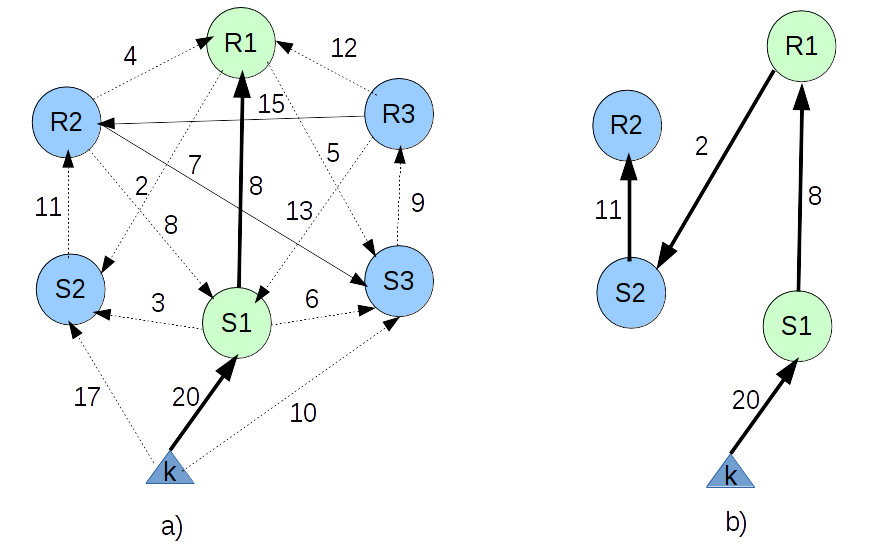
\includegraphics[width=1\linewidth]{images/pict1}}
	\caption{Приклад виконання одного кроку методом Соломона}
	\label{ris:pict1}
\end{figure}

На рис. \ref{ris:pict1} представлений зважений граф, на прикладі якого показано виконання одного кроку методом Соломона:\\
а) вихідний граф, на якому показані варіанти додавання нових заявок на маршрут;\\
b) маршрут, який був побудований методом Соломона після виконання одного кроку.

\textit{Приклад.} Спочатку дана заявка (яка складається з відправника і одержувача). Значення функції вартості $\Omega$ представлені на дугах графа (рис.\ref{ris:pict1}). Необхідно додати нові заявки в маршрут, використовуючи критерії \ref{insert_kr} і \ref{kriterij}. Коефіцієнт $\mu=0.5$.

\textit{Рішення.} Розглянемо процес додавання нових заявок. З двох запропонованих заявок $(\{S_2,R_2\},\{S_3,R_3\})$ виберемо ту, яку потрібно додати в першу чергу. В залежності від місця куди можна додати заявку (початок, кінець, середина) виберемо потрібний критерій. Таким чином, знайдемо оптимальне рішення вставки нової заявки $\{S_2,R_2\}$:\\
$\min[c(k,S_1, \{S_2, R_2\}, R_1), c(k,\{S_2, R_2\}, S_1, R_1), c(k, S_1, R_1, \{S_2, R_2\})]=\min[3+11+4-0.5 \cdot 8; 17+11+8-0.5 \cdot 20; 2+11]=\min[14;26;13]$\\
Знайдемо оптимальне рішення вставки нової заявки $\{S_3,R_3\}$:\\ 
$\min[c(k,S_1, \{S_3, R_3\}, R_1), c(k,\{S_3, R_3\}, S_1, R_1), c(k, S_1, R_1, \{S_3, R_3\})]=\min[6+9+12-0.5 \cdot 8; 10+9+13-0.5 \cdot 20; 5+9]=\min[23;22;14]$.\\
Із знайдених рішень виберемо рішення з найменшим значенням $c(k,v_i,u,v_{i+1})$. У нашому прикладі це $c(k, S_1, R_1, \{S_2, R_2\}=13$.

Таким чином, новий маршрут буде складатися з початкових заявок і нової заявки $\{S_2,R_2\}$, яка буде додана в кінець маршруту.

\textit{Відповідь}: в маршрут $\{S_1,R_1\}$ необхідно додати заявку $\{S_2,R_2\}$, яка буде розміщена в кінці. 

На рис. \ref{ris:pict2} представлені варіанти додавання в маршрут нової заявки $\{S_2,R_2\}$:\\
a) варіант додавання заявки $\{S_2,R_2\}$ в кінець маршруту;\\
b) варіант додавання заявки $\{S_2,R_2\}$ в початок маршруту;\\
c) варіант додавання заявки $\{S_2,R_2\}$ між вершинами $\{S_1,R_1\}$.

На рис. \ref{ris:pict3} представлені варіанти додавання в маршрут нової заявки $\{S_3,R_3\}$:\\
a) варіант додавання заявки $\{S_3,R_3\}$ в кінець маршруту;\\
b) варіант додавання заявки $\{S_3,R_3\}$ в початок маршруту;\\
c) варіант додавання заявки $\{S_3,R_3\}$ між вершинами $\{S_1,R_1\}$.

\begin{figure}[t]
	\center{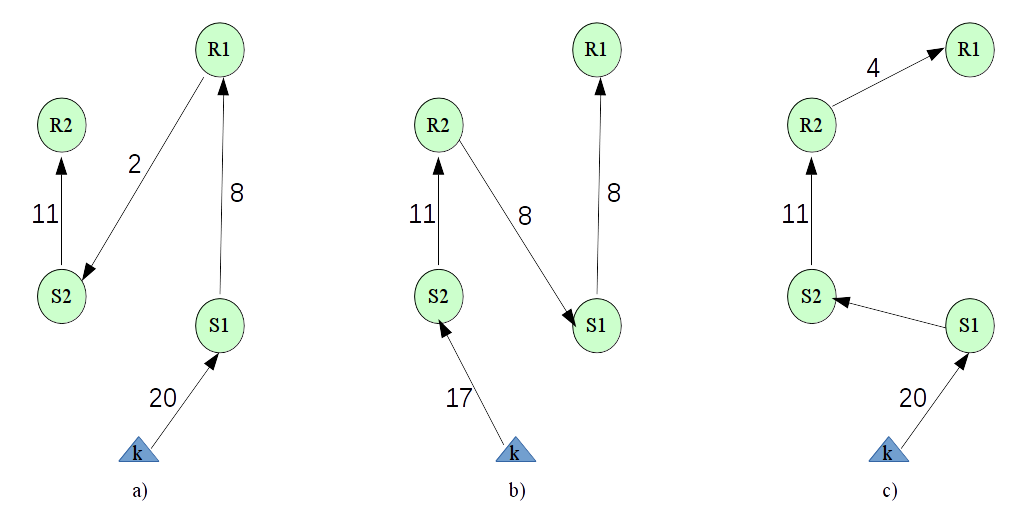
\includegraphics[width=1\linewidth]{images/pict2}}
	\caption{Варіанти додавання в маршрут заявки $\{S_2,R_2\}$}
	\label{ris:pict2}
\end{figure}

\begin{figure}[t]
	\center{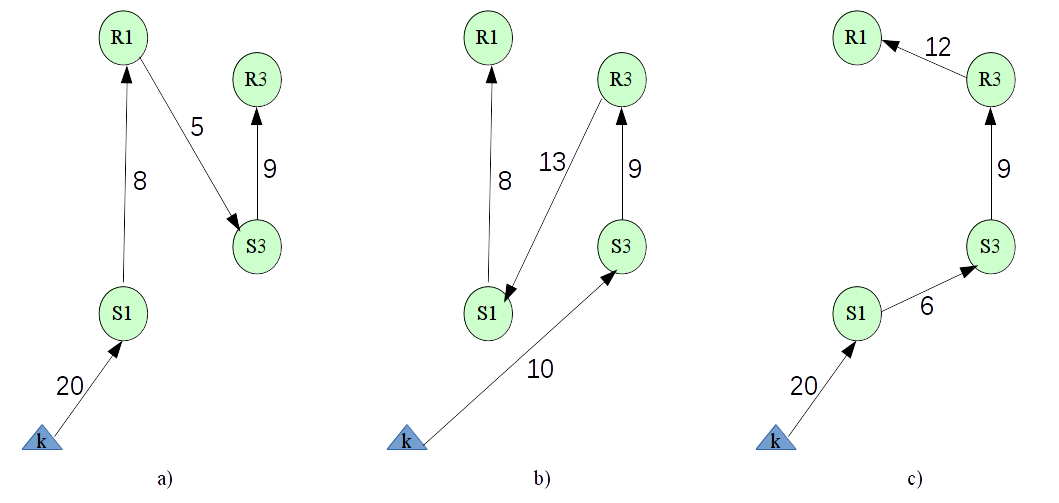
\includegraphics[width=1\linewidth]{images/pict3}}
	\caption{Варіанти додавання в маршрут заявки $\{S_3,R_3\}$}
	\label{ris:pict3}
\end{figure}

\clearpage


\subsection{Метод формування околиці}
Під час роботи алгоритму імітації відпалу необхідно проводити перегляд околиці $N_{l}(\vec{u^i})$ поточної точки $\vec{u^i}$.В ході обчислення маршруту в околицю потрапляє досить велика кількість точок. Але в зв'язку з особливостями обмежень нашої моделі багато з цих точок не є рішенням задачі. Тому в зв'язку з особливостями розглянутої дискретної задачі ми використали наступний прийом визначення околиці.

Нехай $x^{k}(v)$ -- індекс вузла $v$, $v \in R \cup S$ в маршруті автотранспортного засобу $k \in C$. Кожна заявка складається з пари $\{S,R\}$, де $S$ -- це відправник, а $R$ -- одержувач. Під час визначення околиці, повинна зберігатися цілісність маршруту, тобто виконуватися обмеження (\ref{main_cond_1} --\ref{main_cond_4}). Над заявками маршруту $Route_i$, $i=1 \dots n$ виконуються операції перестановки. Отримані під час перестановок вектори $\vec{u}$ і буде околицею $N_{l}(\vec{u^i})$. Для перестановки використовувалися операції переміщення і поглинання.

Операція поглинання представлена на рис.\ref{ris:figures}(a), на якому представлено два маршрути $Route_1$ і $Route_2$. Маршрут $Route_1$ складається з вузлів $\{C_1,S_1,R_1,S_2,\\R_2,S_3,R_3\}$, а маршрут $Route_2$ складається з вузлів $\{C_2,S_4,R_4,S_5,R_5,S_6,R_6\}$. Під час виконання операції поглинання заявки $\{S_1,R_1\}$ в маршруті $Route_1$, вставка даної заявки в маршрут $Route_2$ може бути виконана на $n+1$ позицій. 

\begin{figure}[h]
	\center{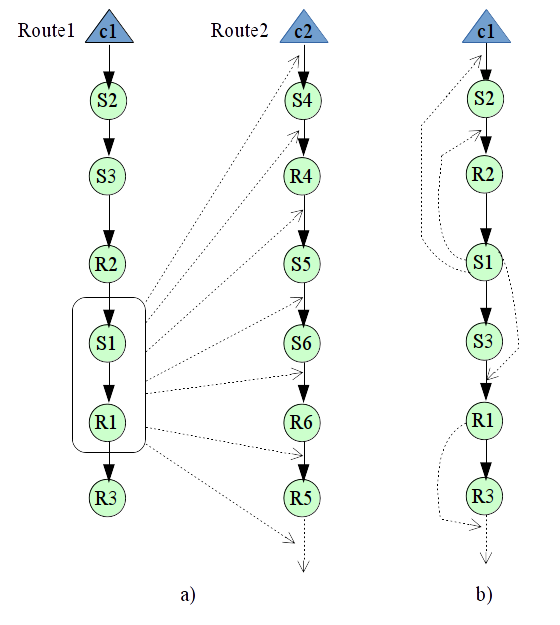
\includegraphics[width=0.75\linewidth]{images/neighboard.png}}
	\caption{Приклад операції a)поглинання та b)переміщення}
	\label{ris:figures}
\end{figure}

Операція переміщення представлена на рис.\ref{ris:figures}(b) На даному рисунку представлений маршрут $Route_1$, який складається з вузлів $\{C_1,S_1,R_1,S_2,R_2,S_3,R_3\}$. Для збереження цілісності маршруту вузол $S_i$ (відправник) має бути відвіданий до $R_i$ (одержувач), виходячи з цього під час операції переміщення, вузол $S_i$ може переміщатися поки буде виконуватися умова $0<x^{new}(S_i)<\widetilde{u}(R_i)$, а вузол $R_i$ може переміщатися поки буде виконуватися умова $n^k \geq x^{new}(R_i)>\widetilde{u}(S_i)$.

\subsection{Analysis of the algorithm parameters}
The Tabu Search algorithm has two main parameters: $h$ -- size of the list of prohibitions and $N_{neighbors}$ -- accepted count limit of size of neighbordhood $N_l(\vec{u})$. For the experiments, we constructed the test tasks on the basis of the capacity routing problems developed by Breedam, Fisher, Christofides and Eilon. To determine trends in time and cost of the decision we used exponential smoothing by a factor of $0.1$.

\begin{figure}[h]
	\hfil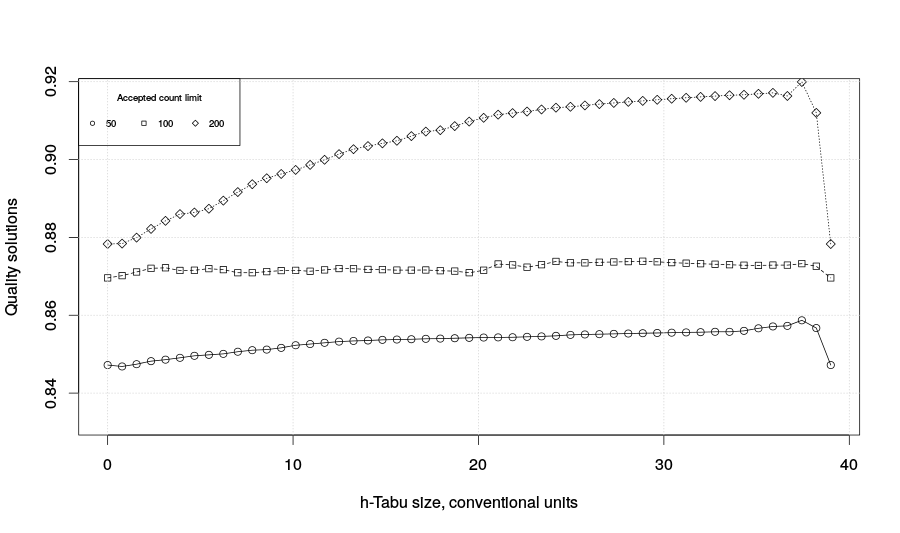
\includegraphics[height=3.0in]{images/tabuSize_stepCount}\hfil
	\caption
	{
	  The dependence of the quality of solutions on the size of the tabu list when using $ StepCount $ termination strategy
	}
	\label{aba:fig2}
\end{figure}

In this experiment we use two different breakpoint strategies: 
\begin{enumerate}
	\item $StepCount$ termination strategy --  terminates when an amount of steps has been reached;
	\item $TimeSpent$ termination strategy -- terminates when an amount of time has been reached.
\end{enumerate}

As should have been expected, for large values of the parameter a jam occurs in local optimum due to the large number of restrictions of movement in space. Otherwise if you select a too small tabu size, algorithm can still get stuck in a local optimum. In the first computational experiment we made finding the best solutions for different values of the tabu size parameter from interval $h \in [0, 40]$ (pict. \ref{aba:fig2} an pict. \ref{aba:fig3}).
\begin{figure}[h]
	\hfil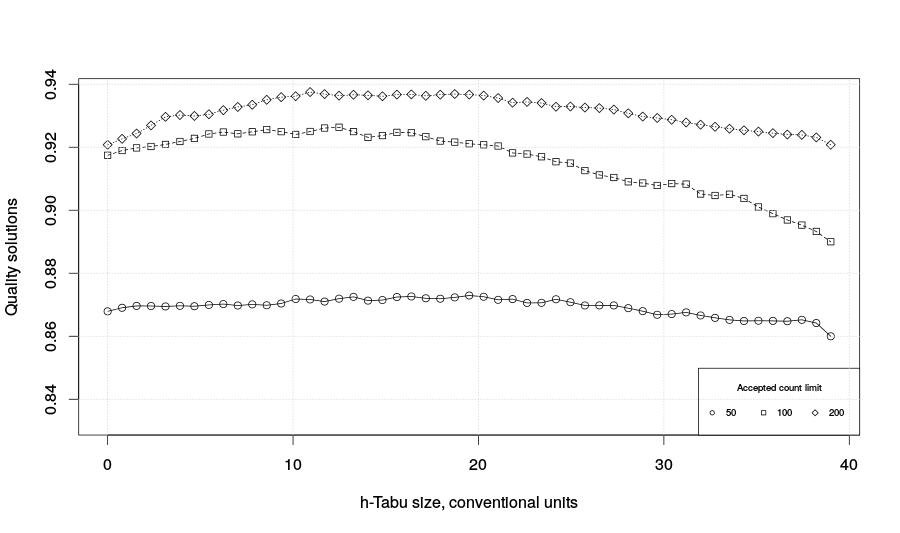
\includegraphics[height=2.2in]{images/tabuSize_time}\hfil
	\caption
	{
	  The dependence of the quality of solutions on the size of the tabu list when using $ TimeSpent $ termination strategy
	}
	\label{aba:fig3}
\end{figure}

\begin{figure}[h]
	\hfil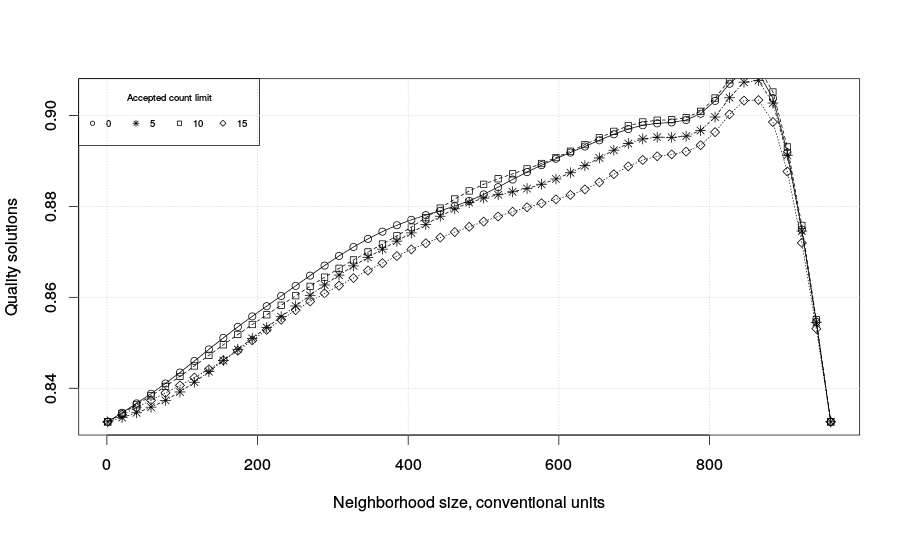
\includegraphics[height=2.2in]{images/acceptedCountLimit}\hfil
	\caption
	{
	  The dependence of the quality of solutions on the neighborhood size when using $ TimeSpent $ termination strategy
	}
	\label{aba:fig4}
\end{figure}

In the second experiment (see figure \ref{aba:fig4}) we built a relationship between the number $N_{neigh.}$ of viewed solutions neighborhood size $N_l(\vec{u})$ using $TimeSpent$ termination strategy. In this experiment we made finding the best solutions for different values of the neighborhood size parameter from interval $N_{neigh.}\in[750, 850]$.

\subsection{Modification}

The first generalized diagram is as follows. First, the set of solutions is constructed by Solomon. Then every solution is improved by tabu search and choose the best solution according to the objective function.

Modification of the scheme is based on the hypothesis of "On a large valley"\cite{opt_Kochetov}. According to this hypothesis, the average local optima are located much closer to the global than a randomly chosen point. There is a certain concentration of local optimum in a small part of the feasible region, which is figuratively called a large valley. If this assumption is true, then it is advisable to remember the best solutions and based on them design new original decision. We use this idea to solve the  Routing Courier Delivery Problem.

We proceed to the description of the algorithm in scheme \ref{alg:constructSolution}. Let $U^{opt}$ is a sorted array of optimal solutions by value of the objective function ascending,  ie:
\begin{equation} \label{u_sorted}
F(u^{opt}_1) \leq F(u^{opt}_2) \leq \ldots < F(u^{opt}_i) \leq \ldots \leq F(u^{opt}_{sizeof(U^{opt})})
\end{equation}
Each solution $u^{opt}_i$ gets into the population with a given probability $p^i_u$, the probability of selection decreases with increasing sequence number:
\begin{equation} \label{p_sorted}
p^1_u = 1 > p^2_u > \ldots > p^i_u> \ldots   > p^{sizeof(U^{opt})}_u,  p^{sizeof(U^{opt})}_u > 0
\end{equation}

\begin{algorithm}[H]

	\textbf{function constructSolution}( $U^{opt}, p_u, n^{min}_s$) \\
	// $U^{opt}$ -- a sorted set array of optimal solutions \\
	
	
	\If{$ sizeof(U^{opt}) <  n^{min}_s$}{
		// construct solution using heuristics(for example, Solomon alg.)\\
		$u^0 = heuristicsConscruction()$ \\
		\textbf{return} $u^0$
	}
	
	\While{$i < sizeof(U^{opt})$}{
		\If{$random(0.0,1.0) > p^i_u$}{
		   i = i + 1 \\
		   \textbf{goto} 8
		}
		$R_i = $randomly select a route from $u^{opt}_i$ solution;
		$u^0 = u^0 \cup R_i$
		i = i + 1\\
		
	}
	
	\If{$u^0 is not complete$}{
	   	$u^0 = heuristicsConscruction(u^0)$
	}
	
	\textbf{return} $u^0$
	
	\caption{Pseudo-code for heuristics construction algorithm.}
	\label{alg:constructSolution}
\end{algorithm}

It then crosses solutions by the following rule: with the first solution is randomly selected route $R_1$. Then another solution is selected from a route $R_2$ that does not include client requests from the first  route etc. If the client requests were not included in the solution $u^0$, then these requests are added by the construction heuristics algorithm (for example, Solomon algorithm).


Now we describe the primary function $SolveCDP()$ of the modified algorithm presented in pseudocode form in Scheme \ref{alg:modTabuSearch}. In this function using a loop is a sequential formation of an array of the best solutions $U^{opt}$ by means TabuSearch algorithm.   

Based on the results of the experiments described in the preceding section, we decided to set the parameters of the algorithm are not fixed values, but as a random variable of predetermined period. For example, the size of the tabu list $h$ is defined as the interval $[10,35]$(see pict. \ref{aba:fig2} and  pict. \ref{aba:fig3}) and the neighbordhood size $l=N_{neighbordhood}$ is defined as the interval $[600\cdot n,850\cdot n]$, where $n$ -- problem size (see pict. \ref{aba:fig4} ).

Let $\vec{\psi_i} = (\psi^1_i,\psi^2_i,\psi^3_i) = (\tilde{l_i},\tilde{p_i},\tilde{l_h})$ -- a set of values of the TabuSearch configuration parameters which was using for solving the problem in the step $i$.

Let $[\psi^j_{begin}, \psi^j_{end}]$ -- an optimal interval of the TabuSearch $j$ -parameter. (For example: if $j=3$, then: $[\psi^3_{begin}, \psi^3_{end}]= [h_{begin}, h_{end}] = [10, 40] $). These intervals are initial data and they are set in the initialization block. 

The configuration parameters  $\psi^j_i $ are randomly selected from the interval $[\psi^j_{begin}, \psi^j_{end}]$ according to a distribution law. We proposed to build the distribution density $f_j(\psi^j_i)$ of the random variable $\psi^j_i$ as follows. At first, we define anchor points:
 
 \begin{equation} \label{anchor_points}
     \rho^j_i =  \dfrac{F(u^{opt}_1)}{avg[F(u^{opt}_k)]}, \forall k: \psi^j_k = \psi^j_i
 \end{equation}
 The number of anchor points $n_{\rho}$  is smaller than the set of optimal solutions, because a set of  anchor points are removed the same points $(n_{\rho} \leq  n_u)$.
 
The main idea is that the distribution density should be larger at those points (parameters $\psi^j_i$) in which high quality solutions than the points at which the low quality of solutions.
Therefore, we presented the distribution function $f_j(z)$ as a sum of kernel functions:
 \begin{equation} \label{dist_density}
 f_j(z) = \alpha_j * \sum\limits_{i=1}^{n_{\rho}}  \rho^j_i * K(z -  \psi^j_i)
 \end{equation}
 where: $K(x)$ -- kernel function, $ \alpha$ -- a normalizing parameter
 
 We have chosen as the kernel the function of parabolic type(known as an Epanechnikov function),  because during the experiments the best results were obtained using this function:
 \begin{equation} \label{dist_density}
  K(z) = 3/4 \cdot (1-z^2)
 \end{equation}
 

\begin{algorithm}[H]
	\textbf{function SolveCDP}( $n^{min}_s$) \\
	// Initialize variables:	\\
	
	$\psi = \emptyset$,
	$p_u = \emptyset$,
	$U^{opt} = \emptyset$,
	$i=0$ \\
	
	\While{the breakpoint is not triggered }{
		// set TabuSearch parameters \\
		\For{$j=1 \ldots 3$}{
	  	// $f_j$ -- the density distribution of the random \\
	  	// variable $\psi^j$ (TabuSearch parameter $l,p $ or $ h$) \\
	  	$\psi^j_i = random(\psi^j_{begin}, \psi^j_{end}, f_j) $
	  	}
	  	
		// Make solution using euristics construction algorithms \\
		$u^0 = constructSolution(U^{opt} ,n^{min}_s)$ 
		
		// Improve solution $u^0$ using TabuSearch algorithm 
		$u^{opt}_i = TabuSearch(u^0, \vec{\psi_i})$ \\
		
		$U^{opt}  = U^{opt} \cup \{u^{opt}_i\}$ \\
		
		// Sort ascending optimums $U$ of the objective function \\
		$U^{opt} = sort(U^{opt})$\\
		$p^{i+1}_u = update(p^i_u)$\\
		
		i = i + 1\\
		
	}
	\textbf{return} $u^{opt}_1$
	
	\caption{Pseudo-code for modified tabu-search algorithm.}
	\label{alg:modTabuSearch}
\end{algorithm}

 The parameter $\alpha_j$ was introduced in the density function to perform the normalization condition:
 \begin{equation} \label{norm_cond}
 \int\limits_{\psi^j_{begin}}^{\psi^j_{end}} f_j(z)dz = 1  =>  (\alpha_j)^{-1} = \sum\limits_{i=1}^{n_{\rho}} \rho^j_i \cdot  \int\limits_{\psi^j_{begin}}^{\psi^j_{end}} K(z -  \psi^j_i) dz 
 \end{equation}

 The parameter $\alpha_j$ can be written in explicit form:
  \begin{equation} \label{norm_cond}
 \begin{split}
 (\alpha_j)^{-1} & = \dfrac{3}{4} \cdot \sum\limits_{i=1}^{n_{\rho}} \rho^j_i \cdot [(1 - (\psi^j_i)^2) \cdot (\psi^j_{end} - \psi^j_{begin}) + \\
 & + \psi^j_i \cdot ((\psi^j_{end})^2 - (\psi^j_{begin})^2) - 1/3 \cdot (\psi^j_{end})^3 - (\psi^j_{begin})^3)]
 \end{split}
 \end{equation}
 
 In figure \ref{aba:fig5} the results of an experiment in which  were presented a dependence of the quality of the solutions obtained by the classical and modified algorithms and  the breaking point time. As seen from the graph, with an increase in operating time of the computational scheme, the quality of solutions obtained using the modified algorithm is growing faster than using classical Tabu Search algorithm.
 
 \begin{figure}[h]
 	\hfil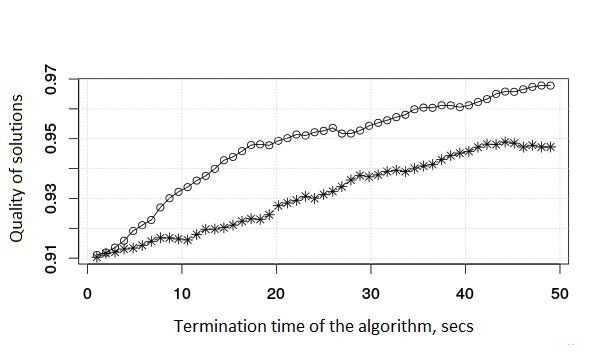
\includegraphics[height=3.0in]{images/tabu_mod.png}\hfil
 	\caption
 	{
 		The dependence of the quality of solutions and  the breaking point time by classic and modified algorithms using $ TimeSpent $ termination strategy
 	}
 	\label{aba:fig5}
 \end{figure}
 
 
\subsection{Conclusion}
During the research has been investigated and implemented tabu search algorithm to solve the Static Routing Courier Delivery problem with time constraints. Also a modified algorithm was developed  based on the Tabu Search algorithm to improve the quality of the solutions. Modified algorithm gave the best solutions in terms of the balance between the number of vehicles and the cost traveled.  In practice this algorithm can be used for decision support in intelligent systems for improving the quality of customer service and for reducing waiting the time to use vehicle, this will reduce fuel costs and depreciation of transport.

The analysis of the parameters of implemented algorithms allowed us to determine their optimal values for this class of routing problems. With the modified algorithm was found solutions of model problems, which in most cases have an acceptable deviation from the global optimum.




\begin{thebibliography}{99}
%In brackets we writes the name which is used for referencing.

\bibitem{RCDS} F.~Ordonez, Chen Wang, A New Approach for Routing Courier Delivery Services //METRANS Transportation Center:University of Southern California
Los Angeles,  2012, 81--115.

\bibitem{Delivery_Masson_2014} R.~Masson, F.~Lehued, O.~ Peton,The dial-a-ride problem with transfers. // Computers and Operations Research, Vol. 41, 2014, p. 12--23.
% http://www.sciencedirect.com/science/article/pii/S0191261599000168

\bibitem{Delivery_Babb_2005} T.~Babb, Pickup and Delivery Problem with Time Windows // Coordinated Transportation Systems: The State of the Art. Department of Computer Science University of Central Florida Orlando, Florida, 2005, 38 p.

\bibitem{vrp_shafeyev} R.~Shafeyev ,L.~Lyubchik, A some realization of Tabu Search algorithm for Solving the Transportation Problem with Time Constraints // Vestnik NTU "KhPI". – Kharkov: NTU
"KhPI", 2013. – No3 (977). – p. 35–39.

\bibitem{jlogistics}  R. Shafeyev. Java-based optimixation framework for solving routing problems.\\ url: http://jlogistics.net, 2015.

\bibitem{Delivery_Barnes_2000} W~Barnes, Solving the pickup and delivery problem with time windows using reactive tabu search // Transportation Research Part B: Methodological, Vol. 34 Issue 2, 2000, p. 107--121.

\bibitem{Delivery_Coltin_2014} B.~Coltin, M.~Veloso, Scheduling for Transfers in Pickup and Delivery Problems with Very Large Neighborhood Search // The Twenty-Eighth Conference on Artificial Intelligence, Quebec City, Canada, 2014, 7 p.
% http://www.cs.cmu.edu/~mmv/papers/14aaai-ColtinVeloso.pdf

\bibitem{opt_Goncharov} E.~Goncharov, Y~Kochetov, Probabilistic search with exclusions for discrete unconstrained optimization  //Discrete Analysis and Operations Research, Moscow, Serial 2. Vol. 9, 2002, p. 13-30.
%Гончаров Е.Н., Кочетов Ю.А. Вероятностный поиск с запретами для дискретных задач безусловной оптимизации // Дискрет. анализ и исслед. операций. Сер. 2. Т.9, № 2. 2002, с. 13-30.

\bibitem{opt_Kochetov}   Y~Kochetov, Probabilistic methods of local search for discrete optimization problems //Discrete Mathematics and Its Applications: Proceedings of youth lectures and scientific schools in discrete mathematics and its applications, Publishing House of the Center for Applied Research at the Mechanics and Mathematics. Faculty of Moscow State University, 2001, p. 84-117.  
%Кочетов Ю.А. Вероятностные методы локального поиска для задач дискретной оптимизации // Дискретная математика и ее приложения: Сб. лекций молодежных и научных школ по дискретной математике и ее приложениям. М.: Изд-во центра прикл. исслед. при мех-мат. фак. МГУ, 2001, с. 84-117; 

\bibitem{Tabu_search} O.~Braysy, M.~Gendreau, Vehicle Routing Problem with Time Windows, Part I: Route Constuction and local algorithms // Transportation science Vol.39 No. 1, 2005, p. 104-118.

\bibitem{Goldberg_Kennedy} V.~Goldberg, R.~Kennedy, An Efficient cost scaling algotirhm for the assignment problem, Math. Program., 1995, p. 153--177.  

\bibitem{problems_Christofides}  N. Christofides, S. Eilon, An algorithm for the vehicle dispatching problem //Operational Research Quarterly, 20, 1969, p. 309–318.

\bibitem{problems_Golden}  B. Golden, E. Wasil, J. Kelly, I-M. Chao. The impact of metaheuristics on solving the vehicle routing problem: Algorithms, problem sets, and computational results. In T. Crainic and G. Laporte, editors // Fleet Management and Logistics, Kluwer, Boston, 1998 p. 33–56.

\bibitem{problems_Taillard}  E. Taillard. VRP benchmarks.\\ url: http://mistic.heig-vd.ch/taillard/problemes.dir/vrp.dir/vrp.html, 1993.

\bibitem{Attanasio} A.~Attanasio, J.~Bregman,G.~Ghiani, E.~Manni. Real-time fleet management at Ecourier Ltd. Dynamic Fleet Management, volume 38 of Operations Research/Computer Science Interfaces, chapter 10, p.219--238, 2007.

\bibitem{Beaudry} A.~Beaudry, G.~Laporte, T.~Melo, Nickel. Dynamic transportation of patients in hospitals. Berichte des Fraunhofer ITWM, Nr. 104 :p.1--34, 2010.

\bibitem{Romero} M.Romero, L.Sheremetov and A.Soriano. A genetic algorithm for the pickup and delivery problem: An application to the helicopter offshore transportation. In Theoretical Advances and Applications of Fuzzy Logic and Soft Computing, volume 42 of Advances in Soft Computing, 2007, p. 35--44.

\bibitem{Kergosien} M.Romero, L.Sheremetov and A.Soriano. Yannick Kergosien, Christophe Lent, D. Piton, Jean-Charles Billaut. A tabu search heuristic for a dynamic transportation problem of patients between care units. 29 pages. 2010.

\bibitem{Sarak} H.~Sarak, A.~Satman. The degree-day method to estimate the residential heating natural gas consumption in Turkey: a case study. Pergamon, Energy 28 (2003) 929--939.
	
\end{thebibliography}



\end{document} \grid
\grid
